\section{Related Work}
\label{sec:survey:related-work}

% Discuss identified related work
% - Service Mesh survey
% - Our previously conducted survey on the k8s ecosystem
Prior to conducting a survey on the field, we examined relevant and related work on the topic. We have identified secondary literature in which authors have conducted a literature review on the state-of-the-art on \gls{sm} technology \cite{service-mesh-survey}. This review that was conducted in 2019 noted the fact that there was not a lot of formal literature on the topic and stated that their work was the first work to formally synthesize the data in the field. Previous efforts by us to systematically synthesize the data concerning the formal literature on the \gls{k8s} ecosystem found similar results. \todo{Survey: Cite prev work?} In our previous work, we presented a topical framework on research conducted in the Kubernetes ecosystem and found that most of the formal literature was related to the resource management aspects of the ecosystem. With most of the research dedicated to scheduling and scaling algorithms, several of the layers as presented in the topical framework \todo{add ref to frameowkr} had relatively little attention. One of the identified technologies that was related to the Kubernetes ecosystem, in the form of \glspl{sm}, had very little formal work conducted on it, which ultimately led to the motivation behind the research conducted in this thesis.

% Reason the need for such a survey
% - Previous attempt gave general introduction
% - Not a sytems survey
% - Comparison of only a few (Istio, Linkerd, App Mesh, Synapse) sm implementations
% - Landscape changed, new technolgies, definition might change?
Although there has been a previous effort to survey the field \cite{service-mesh-survey}, we identified several shortcomings for our goals. First, the survey conducted by Li et al. provide a generic introduction to the concept of a service mesh, its features, and the challenges and opportunities in the field. Our goal is to provide a comparison of \gls{sm} implementations through their characteristics and properties. The work conducted by Li et al. do provide some form of comparison, but do so with a focus on generic and subjective characteristics such as the maturity of the product, whether it is open-source and actively worked on and what the major advantage and disadvantage is of each platform. This provides a sharp contrast in the type of comparison that we try to conduct, which heavily emphasizes on characteristics typically associated with  \gls{sm} technologies detailing the control and data plane characteristics of such a system. Furthermore, the survey was conducted in 2019, however the landscape of \gls{sm} technologies has changed drastically since then. New \gls{sm} systems have emerged, while existing systems have evolved. Where Li et al. \cite{service-mesh-survey} have identified four different systems back in 2009, the \gls{cncf} landscape \cite{cncf-landscape}\footnote{\url{https://landscape.cncf.io/card-mode?category=service-mesh&grouping=category}} contains many more systems as is depicted in \cref{fig:cncf-landscape-sm}. This landscape only presents officially accepted \gls{cncf} projects and might not cover all the systems which are out there. Finally, recent industry based efforts altered some ideas and principles of \gls{sm} systems, changing the traditional proxy-based approaches to include  \gls{ebpf}\footnote{\url{https://ebpf.io/}} based solutions, drastically changing the data plane by including revolutionary Linux kernel technologies \cite{istio-merbridge, cilium-ebpf-mesh}.


\begin{figure*}[t]
    \centering
    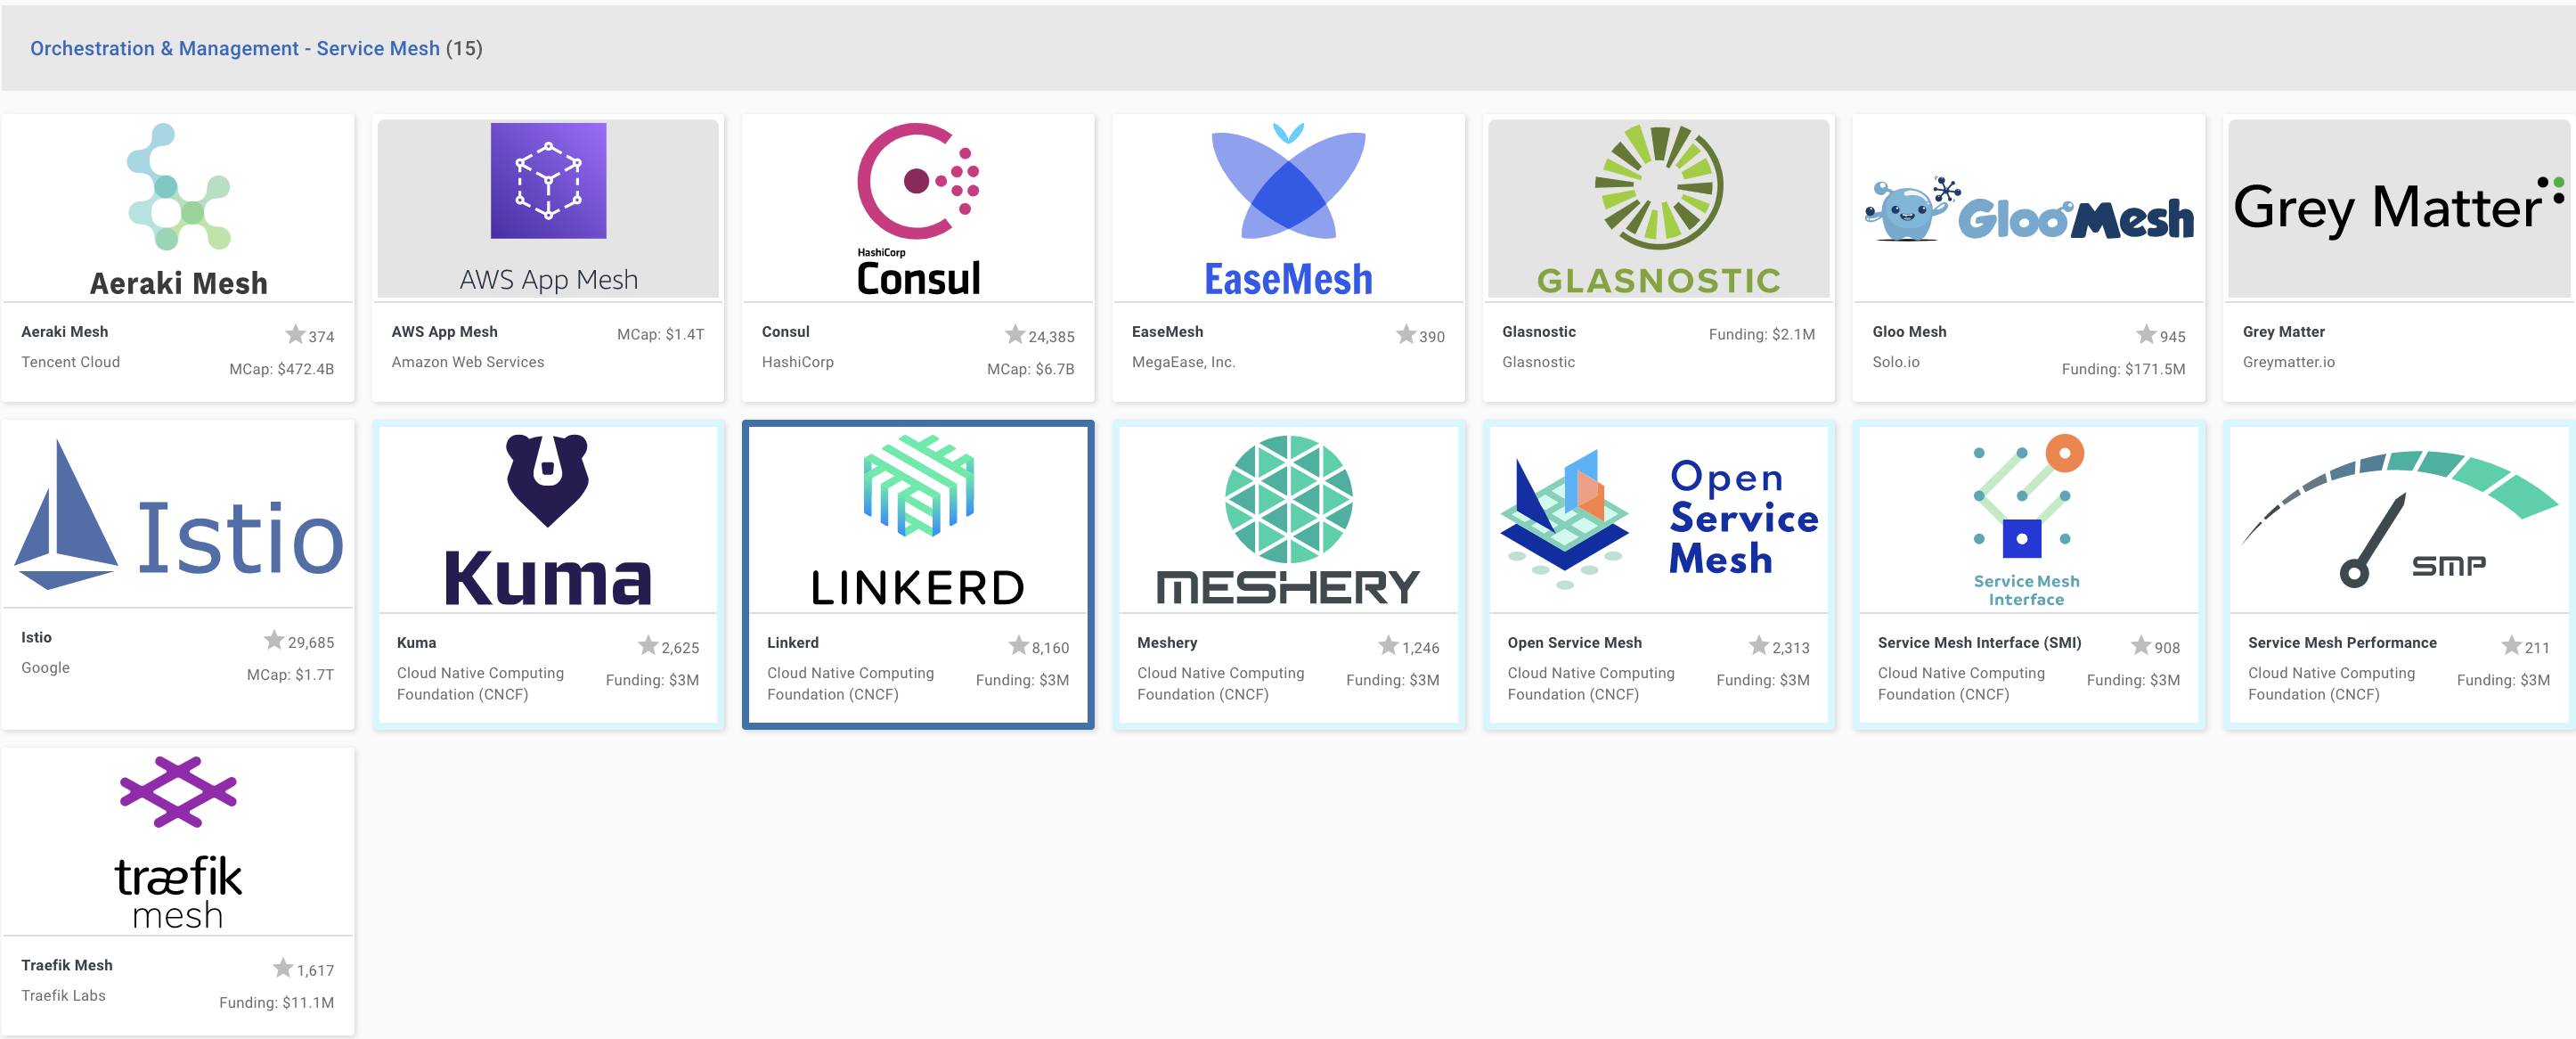
\includegraphics[width=0.9\linewidth]{3_systems_survey/figures/cncf-landscape-service-mesh}
    \caption{\gls{cncf} landscape of \gls{sm} technologies as of March 2022}
    \label{fig:cncf-landscape-sm}
\end{figure*}

% Conclude that there is a need for the review
% - Lack of formal (reiterate)
% - Industry interest
% - New approaches (proxyless, ebpf)
In order to justify a formal systematic survey, we have to evaluate the environment and related work. First, we have evaluated the existing formal literature in the field, as stated above, and concluded that this was lacking and unfit for the goals and research that we have in mind. Secondly, we evaluated the interest from within the community regarding the \gls{sm} technology. Our preliminary analysis showed that this was a sharp contrast against the interest from within the academic world. The field has an abundance of blog posts, talks, and the author of \gls{linkerd}, a popular \gls{sm} implementation, even went as far to call it “the world’s most over-hyped technology” \cite{service-mesh-hype}. Additionally, we found that the technology has received widespread adoption and interest from the industry, with a steady increase in production usage as indicated in surveys conducted by Red Hat \cite{rh-survey} and the \gls{cncf} \cite{cncf-survey-2020}. Finally, the very recent developments \cite{istio-merbridge, cilium-ebpf-mesh} in the field (less than two months old at the time of writing), which fundamentally change the approach, provide  interesting takes to survey this field at this very moment. This all results in a justification for conducting the survey, and that the timing of it manages to capture an interesting shift within the field.

